\documentclass[11pt,a4paper,titlepage,oneside]{book}
%\documentclass[11pt,a4paper,titlepage,twoside]{book}

\usepackage{graphicx}
\usepackage[ruled,linesnumbered,lined,resetcount,algochapter]{algorithm2e}
% Note that IEEE does not support algorithm2e by default
\usepackage{amssymb}
\usepackage{amsmath}
\usepackage{amsfonts}
\usepackage{amsthm} % For typesetting theorems (AMS style)
\usepackage[usenames,dvipsnames]{xcolor}% for set the font color
\usepackage{graphicx}
\usepackage{epstopdf} % Let pdfLatex accept EPS files
\usepackage{array}
\usepackage{color}
\usepackage{pdfpages}
\usepackage[caption=false,font=footnotesize]{subfig}
\usepackage{comment} % To comment some blocks
\usepackage{multirow}
\usepackage{cite}
\usepackage{appendix} 
\usepackage{tablefootnote}
\usepackage[nottoc]{tocbibind} % Add lof, lot into toc
\usepackage[colorlinks=false]{hyperref} % Can comment this
\usepackage{listings} % display source code
\definecolor{codegreen}{rgb}{0,0.6,0}
\definecolor{codegray}{rgb}{0.5,0.5,0.5}
\definecolor{codepurple}{rgb}{0.58,0,0.82}
\definecolor{backcolour}{rgb}{0.95,0.95,0.92}
 
\lstdefinestyle{mystyle}{
    backgroundcolor=\color{backcolour},   
    commentstyle=\color{codegreen},
    keywordstyle=\color{magenta},
    numberstyle=\tiny\color{codegray},
    stringstyle=\color{codepurple},
    basicstyle=\footnotesize,
    breakatwhitespace=false,         
    breaklines=true,                 
    captionpos=b,                    
    keepspaces=true,                 
    numbers=left,                    
    numbersep=5pt,                  
    showspaces=false,                
    showstringspaces=false,
    showtabs=false,                  
    tabsize=2
}
 
\lstset{style=mystyle} % settings for listings package
\newcommand{\addcolor}[1]{{\color{blue}#1}} %color font
\newcommand{\notecolor}[1]{{\color{red}#1}} %color font

%For paper, you can let the counter start at each section
\newtheorem{theorem}{Theorem}[chapter]
\newtheorem{problem}{Problem}[chapter]
\theoremstyle{definition}
\newtheorem{definition}{Definition}[chapter]
\theoremstyle{remark}
\newtheorem*{remark}{Remark}%Unnumbered 

% For lab' thesis
\textwidth 160.0 mm
\textheight 220.0 mm
\topmargin -3.0 mm
\oddsidemargin 4.0 mm
\evensidemargin -6.0 mm

\setcounter{secnumdepth}{3}
\renewcommand{\baselinestretch}{1.4}
\pagestyle{plain}



\begin{document}

\includepdf[pages=1]{cover.pdf}
%\includepdf[pages=1]{frontmatter/Library_author_new.pdf}
%\includepdf[pages=1]{frontmatter/Library_extend.pdf}
%\includepdf[pages=1]{frontmatter/advisor_ch.pdf}
%\includepdf[pages=1]{frontmatter/advisor_en.pdf}
%\includepdf[pages=1]{frontmatter/Committee_ch.pdf}
%\includepdf[pages=1]{frontmatter/Committee_en.pdf}
\frontmatter


%\includepdf[pages={1,2},addtotoc={1,chapter,1,Abstract (Chinese),p1},pagecommand={\thispagestyle{plain}}]{frontmatter/abstractCH.pdf}

\begin{center}
{\LARGE \textbf{Abstract} }
\end{center}
\addcontentsline{toc}{chapter}{Abstract (English)}


Lorem ipsum dolor sit amet, consectetur adipisicing elit, sed do eiusmod tempor incididunt ut labore et dolore magna aliqua. Ut enim ad minim veniam, quis nostrud exercitation ullamco laboris nisi ut aliquip ex ea commodo consequat. Duis aute irure dolor in reprehenderit in voluptate velit esse cillum dolore eu fugiat nulla pariatur. Excepteur sint occaecat cupidatat non proident, sunt in culpa qui officia deserunt mollit anim id est laborum.

%\includepdf[pages={1},addtotoc={1,chapter,1,Acknowledgement,p2},pagecommand={\thispagestyle{plain}}]{frontmatter/acknowledge.pdf}

%%Except for english abstract, other documents are external pdf files.


\tableofcontents % toc
\listoffigures % lof
\listoftables % lot
\mainmatter\setcounter{page}{1}

\chapter{First step}
\label{intro}


First, download and install the {\TeX}/{\LaTeX} distribution:
\begin{itemize}
\item MiKTeX (\url{https://miktex.org/})
\item Tex live(\url{https://www.tug.org/texlive/})
\item MacTeX (\url{https://www.tug.org/mactex/}), Mac OS only.
\end{itemize}

Although those {\TeX}/{\LaTeX} distributions all include a {\LaTeX} editor, I prefer use Texmaker(\url{http://www.xm1math.net/texmaker/}) or TeXstudio (\url{https://www.texstudio.org/}).

Then, we can create a document in {\LaTeX}.

\begin{lstlisting}[language=Tex]
\documentclass{article}
\begin{document}
This is hello {\LaTeX} !.
\end{document}
\end{lstlisting}

Save those code into a file with the extension \notecolor{.tex}, e.g., helloworld.tex. and open it with Texmaker.
Follow the steps shown in Figure \ref{fig.latex}, we can obtain the result .pdf file.
First, we use {\LaTeX} to compile this .tex file to generate a .dvi file.
Next, we use \notecolor{DVI$->$PDF} to convert .dvi to .pdf file.
Or, we can use PDFLaTeX to generate the pdf file directly as depicted in Figure \ref{fig.pdflatex}.
Then, we can view the pdf file by the built-in viewer.


\begin{figure*}[!t]
\centering
\subfloat[LaTeX]{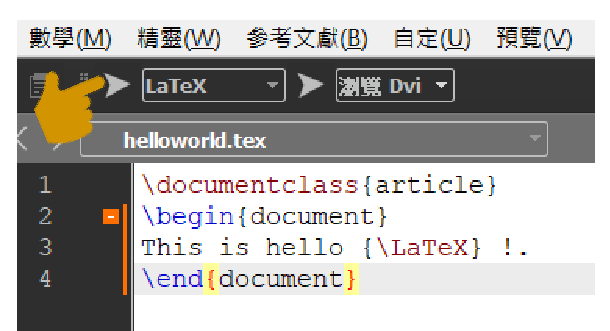
\includegraphics[width= 2.3in]{figs//s1}}
\subfloat[DVI to PDF]{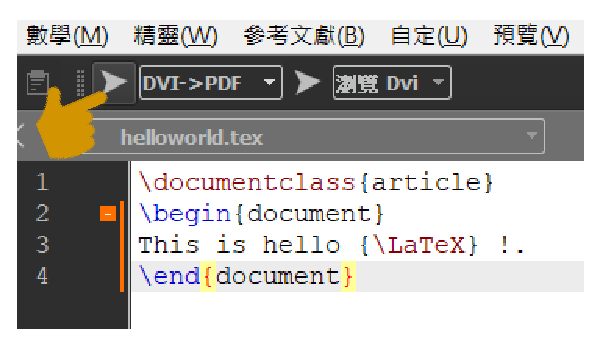
\includegraphics[width= 2.3in]{figs//s2}}
\subfloat[View PDF]{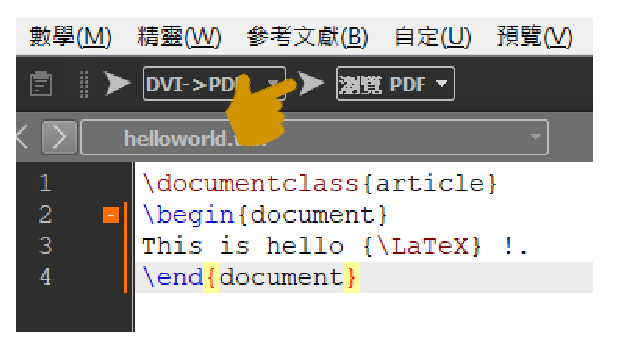
\includegraphics[width= 2.3in]{figs//s3}}
\caption{The basic procedure for LaTeX.}%
\label{fig.latex}%
\end{figure*}


\begin{figure*}[!t]
\centering
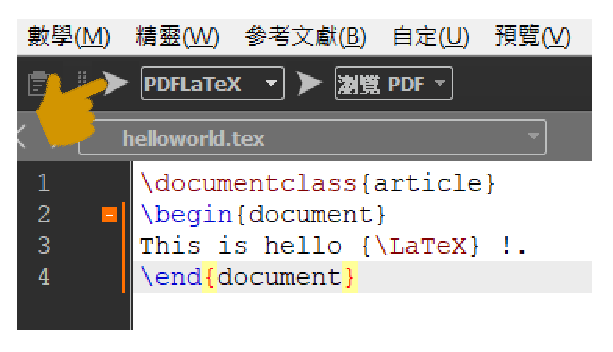
\includegraphics[width= 2.3in]{figs//s4}
\caption{The basic procedure for PDFLaTeX.}%
\label{fig.pdflatex}%
\end{figure*}



Now, go to this website (\url{https://www.sharelatex.com/learn}) to learn the basic knowledge of {\LaTeX}.

\section{Other resources}

\begin{itemize}
\item \url{https://en.wikibooks.org/wiki/LaTeX}
\item \url{https://tex.stackexchange.com/}
\end{itemize}



\chapter{Thesis Template}

This file is a {\LaTeX} thesis template for NCLab's thesis.
The member should review the source file.
The source of this template can be downloaded at : \url{https://github.com/FrankYFHsu/LatexTemplate}

\section{Main part}
The following code is the source code of the main part of this template file.
\lstinputlisting[language=Tex]{thesis_template.tex}


\section{Bibliography and Citation}

Usually, to generate the bibliography, we need to prepare a bibtex (.bib) file that provides information of references.
Bibtex \url{http://www.bibtex.org/Using/} is a format, it looks like 
\lstinputlisting[language=Tex]{bib_example.bib}
Then, we save this content as a .bib file.

The type InProceedings is for conference paper and Article is for journal paper. You can google their difference.
The term such as KarPower2010 is a citation-key or also called BibTeX key that we use it to identify those references.
My personal rule to define the key for a reference is: The first 3 characters of the first author’s last name $+$ The first word of the title $+$ The publication year.

Usually, IEEE xplore, ACM digital library, google scholar provide the paper information in BibTeX format.
Whatever, you need to modify those BibTeX as some entries may not be correct.

Then, before the end of document, we will insert two commands such as:
\begin{lstlisting}[language=Tex]
\bibliographystyle{IEEEtran} % Usually we follow IEEE style
\bibliography{bib_example}
\end{lstlisting}

So, to cite some references like \cite{KarPower2010} or \cite{LeeSLAW2009,ChoFriendship2011,WhiTemporal2012},
the source is:
\begin{lstlisting}[language=Tex]
\cite{KarPower2010} or \cite{LeeSLAW2009,ChoFriendship2011,WhiTemporal2012}
\end{lstlisting}


Note that, if we change the citation or bib file, or we are first time to generate bibliography, we need to compile our .tex file by bibtex.
The overall process is: (1)PDFLaTeX, (2)BibTex, (3)PDFLaTeX, (4)PDFLaTeX.


\section{Example of Figures}


\begin{figure}[!tb]
\centering
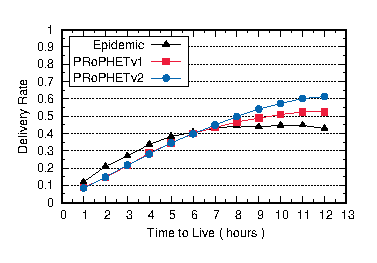
\includegraphics[width=3.4in]{figs//Rate50k.eps}
\caption{Example of a single figure}
\label{fig.1}
\end{figure}

Fig. \ref{fig.1} is an example of a single figure. The source is:
\begin{lstlisting}[language=Tex]
\begin{figure}[!tb]
\centering
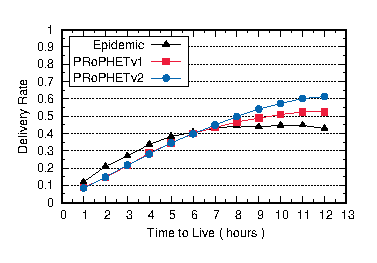
\includegraphics[width=3.4in]{figs//Rate50k.eps}
\caption{Example}
\label{fig.1}
\end{figure}
\end{lstlisting}

\begin{figure*}[!tb]
\centering
\subfloat[Delivery rate]{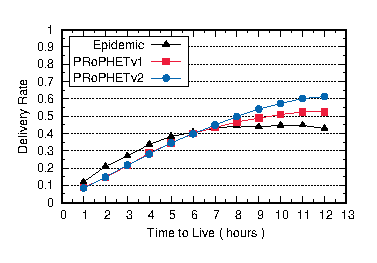
\includegraphics[width= 2.2in]{figs//Rate50k.eps}}
\subfloat[Overhead]{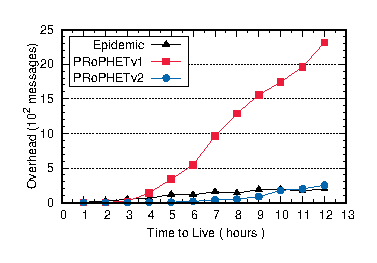
\includegraphics[width= 2.2in]{figs//Overhead50k.eps}}
\subfloat[Latency]{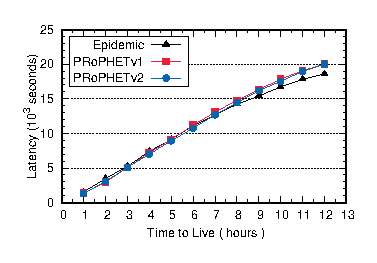
\includegraphics[width= 2.2in]{figs//Latency50k.eps}}\\
\subfloat[Delivery rate]{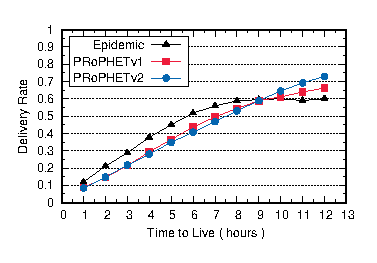
\includegraphics[width= 2.2in]{figs//Rate100k.eps}}
\subfloat[Overhead]{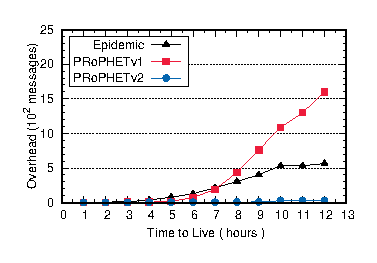
\includegraphics[width= 2.2in]{figs//Overhead100k.eps}}
\subfloat[Latency]{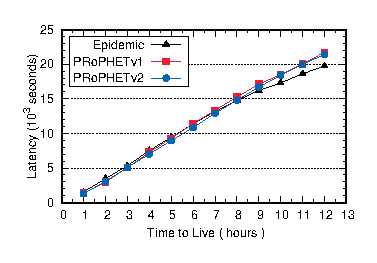
\includegraphics[width= 2.2in]{figs//Latency100k.eps}}
\caption{Example of sub figures}%
\label{fig.2}%
\end{figure*}


Fig. \ref{fig.2} is an example of subfigures. The source is:
\begin{lstlisting}[language=Tex]
\begin{figure*}[!tb]
\centering
\subfloat[Delivery rate]{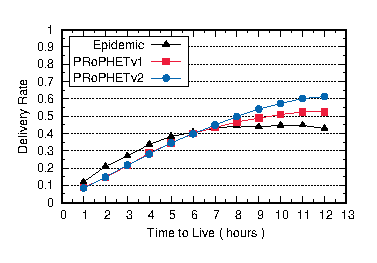
\includegraphics[width= 2.3in]{figs//Rate50k.eps}}
\subfloat[Overhead]{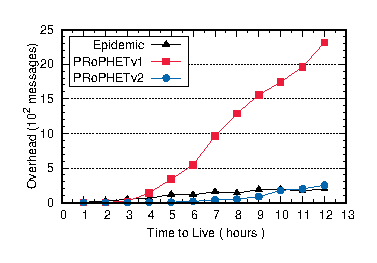
\includegraphics[width= 2.3in]{figs//Overhead50k.eps}}
\subfloat[Latency]{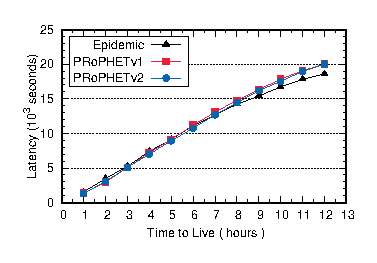
\includegraphics[width= 2.3in]{figs//Latency50k.eps}}\\
\subfloat[Delivery rate]{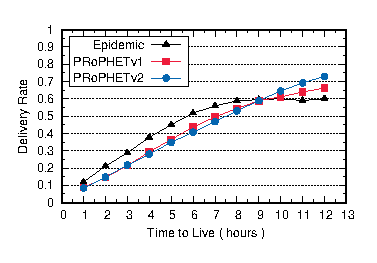
\includegraphics[width= 2.3in]{figs//Rate100k.eps}}
\subfloat[Overhead]{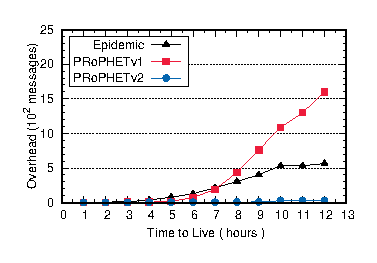
\includegraphics[width= 2.3in]{figs//Overhead100k.eps}}
\subfloat[Latency]{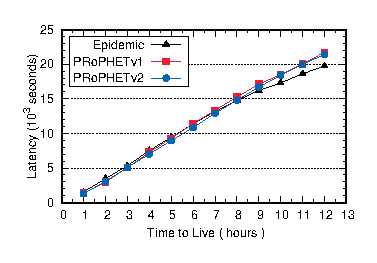
\includegraphics[width= 2.3in]{figs//Latency100k.eps}}
\caption{Example figures. (a)--(c) 50k case and (d)--(f) 100k case.}%
\label{fig.2}%
\end{figure*}
\end{lstlisting}

To reference a figure, you need to set the label of that figure (by the way, you can set the label of table, equation, chapter, section, definition, etc.).
Then, use the command $\setminus$ref$\{label\}$. For example,
\begin{lstlisting}[language=Tex]
As shown in Fig. \ref{fig.1} and Fig. \ref{fig.2}, ....
\end{lstlisting}



%\pagebreak

\section{Example of Table}

\begin{table}[!tb]
\renewcommand{\arraystretch}{1}
\caption{An Example of a Table}
\label{table1}
\centering%
\begin{tabular}{|l|l|}
\hline
Symbol & Meaning \\ \hline
$L$ & Node population, the amount of nodes in a network \\
$B$ & Buffer size, the number of messages that a node can store at most. \\
$R_i$ & Remaining time-to-live (TTL) value for message $i$\\
$M_i$ & Any distinct message $i$ in a network\\
$T_i$ & Elapsed time from the creation of a distinct message $i$.\\
$K(t)$ & The number of distinct messages in a network at time $t$\\
$\vert K\vert$ & The total of distinct messages that were ever created in a network\\
$\lambda$ & Meeting rate between two nodes\\
\hline
\end{tabular}%
\end{table}

\begin{table}[!tb]
\renewcommand{\arraystretch}{1}
\caption{An Example of a Table}
\label{table2}
\centering%
\begin{tabular}{lp{10cm}}
\hline
Symbol & Meaning \\ \hline
$L$ & Node population, the amount of nodes in a network \\
$B$ & Buffer size, the number of messages that a node can store at most. \\
$R_i$ & Remaining time-to-live (TTL) value for message $i$\\
$M_i$ & Any distinct message $i$ in a network\\
$T_i$ & Elapsed time from the creation of a distinct message $i$.\\
$K(t)$ & The number of distinct messages in a network at time $t$\\
$\vert K\vert$ & The total of distinct messages that were ever created in a network\\
$\lambda$ & Meeting rate between two nodes\\
\hline
\end{tabular}%
\end{table}

The source to create Table \ref{table1} and Table \ref{table2}:

\begin{lstlisting}[language=Tex]
\begin{table}[!tb]
\renewcommand{\arraystretch}{1}
\caption{An Example of a Table}
\label{table1}
\centering%
\begin{tabular}{|l|l|}
\hline
Symbol & Meaning \\ \hline
$L$ & Node population, the amount of nodes in a network \\
$B$ & Buffer size, the number of messages that a node can store at most. \\
$R_i$ & Remaining time-to-live (TTL) value for message $i$\\
$M_i$ & Any distinct message $i$ in a network\\
$T_i$ & Elapsed time from the creation of a distinct message $i$.\\
$K(t)$ & The number of distinct messages in a network at time $t$\\
$\vert K\vert$ & The total of distinct messages that were ever created in a network\\
$\lambda$ & Meeting rate between two nodes\\
\hline
\end{tabular}%
\end{table}
\end{lstlisting}

\begin{lstlisting}[language=Tex]
\begin{table}[!tb]
\renewcommand{\arraystretch}{1}
\caption{An Example of a Table}
\label{table2}
\centering%
\begin{tabular}{lp{8cm}}
\hline
Symbol & Meaning \\ \hline
$L$ & Node population, the amount of nodes in a network \\
$B$ & Buffer size, the number of messages that a node can store at most. \\
$R_i$ & Remaining time-to-live (TTL) value for message $i$\\
$M_i$ & Any distinct message $i$ in a network\\
$T_i$ & Elapsed time from the creation of a distinct message $i$.\\
$K(t)$ & The number of distinct messages in a network at time $t$\\
$\vert K\vert$ & The total of distinct messages that were ever created in a network\\
$\lambda$ & Meeting rate between two nodes\\
\hline
\end{tabular}%
\end{table}
\end{lstlisting}

Similar to figures, use the command $\setminus$ref$\{label\}$ to reference a table.
\begin{lstlisting}[language=Tex]
The source to create Table \ref{table1} and Table \ref{table2}:
\end{lstlisting}

\section{Example of Theorem, Problems and Definition}
Defined these commands before $\setminus$begin$\{document\}$
\begin{lstlisting}[language=Tex]
\usepackage{amsthm}
\newtheorem{theorem}{Theorem}[chapter]
\newtheorem{problem}{Problem}[chapter]
\theoremstyle{definition}
\newtheorem{definition}{Definition}[chapter]
\theoremstyle{remark}
\newtheorem*{remark}{Remark}%Unnumbered 
\end{lstlisting}

\begin{theorem}[Theorem 1]
\label{Theorem1}
This is Theorem 1.
\end{theorem}

\begin{problem}[Problem 1]
\label{Problem1}
This is problem 1.
\end{problem}

\begin{definition}[Definition 1]
\label{Definition1}
This is Definition 1.
\end{definition}

\begin{remark}
This is Remark 1.
\end{remark}

The source:
\begin{lstlisting}[language=Tex]
\begin{theorem}[Theorem 1]
\label{Theorem1}
This is Theorem 1.
\end{theorem}

\begin{problem}[Problem 1]
\label{Problem1}
This is problem 1.
\end{problem}

\begin{definition}[Definition 1]
\label{Definition1}
This is Definition 1.
\end{definition}

\begin{remark}
This is Remark 1.
\end{remark}
\end{lstlisting}
Reference: {\url{https://www.sharelatex.com/learn/latex/Theorems_and_proofs}}
\chapter{Equations}

\begin{enumerate}
\item equation+aligned
\begin{equation}
\begin{aligned}
& \text{minimize}
& & C=\sum_{i,j=1}^{n}c_{ij}x_{ij} \\
& \text{subject to}
& & \sum_{i,j=1}^{n}x_{ji}+b_{i}=\sum_{i,j=1}^{n}x_{ij},\; 1^{T}b=0 \\
&&& l_{ij}\leq x_{ij}\leq u_{ij}.
\end{aligned}
\end{equation}
\begin{lstlisting}[language=Tex]
\begin{equation}
\begin{aligned}
& \text{minimize}
& & C=\sum_{i,j=1}^{n}c_{ij}x_{ij} \\
& \text{subject to}
& & \sum_{i,j=1}^{n}x_{ji}+b_{i}=\sum_{i,j=1}^{n}x_{ij},\; 1^{T}b=0 \\
&&& l_{ij}\leq x_{ij}\leq u_{ij}.
\end{aligned}
\end{equation}
\end{lstlisting}

\item align
\begin{align}
& \text{minimize}
& & c^{T}x+b \\
& \text{subject to}
& & Gx\preceq h \\
&&& Ax=b,
\end{align}

\begin{lstlisting}[language=Tex]
\begin{align}
& \text{minimize}
& & c^{T}x+b \\
& \text{subject to}
& & Gx\preceq h \\
&&& Ax=b,
\end{align}
\end{lstlisting}

\item align+aligned
\begin{align}
\begin{aligned}
& \text{minimize}
& & c^{T}x+b \\
& \text{subject to}
& & Gx\preceq h \\
&&& Ax=b,
\end{aligned}
\end{align}

\begin{lstlisting}[language=Tex]
\begin{align}
\begin{aligned}
& \text{minimize}
& & c^{T}x+b \\
& \text{subject to}
& & Gx\preceq h \\
&&& Ax=b,
\end{aligned}
\end{align}
\end{lstlisting}

\item align
\begin{align}
\max\limits_{n_1,n_2,...,n_k}
&\text{\quad}\sum_{i=1}^{K}(1-\text{exp}(-\lambda n_i R_i)),\label{eq1}\\
\text{subject to}
&\text{\quad}\sum_{i=1}^{K}n_ix-LB \leq 0,\label{eq2}\\
&\text{\quad} n_i-L \leq 0,\forall i,\label{eq3}\\
&\text{\quad} n_i \geq 1, \forall i.\label{eq4}
\end{align}

\begin{lstlisting}[language=Tex]
\begin{align}
\max\limits_{n_1,n_2,...,n_k}
&\text{\quad}\sum_{i=1}^{K}(1-\text{exp}(-\lambda n_i R_i)),\label{eq1}\\
\text{subject to}
&\text{\quad}\sum_{i=1}^{K}n_ix-LB \leq 0,\label{eq2}\\
&\text{\quad} n_i-L \leq 0,\forall i,\label{eq3}\\
&\text{\quad} n_i \geq 1, \forall i.\label{eq4}
\end{align}
\end{lstlisting}

\item align$^{\ast}$
\begin{align*}
L(x,\lambda ,\nu )& =c^{T}x+\lambda ^{T}(Gx-h)+\nu ^{T}(Ax-b) \\
& =(c^{T}+\lambda^{T}G+\nu ^{T}A)x-\lambda ^{T}h-\nu ^{T}b.
\end{align*}

\begin{lstlisting}[language=Tex]
\begin{align*}
L(x,\lambda ,\nu )& =c^{T}x+\lambda ^{T}(Gx-h)+\nu ^{T}(Ax-b) \\
& =(c^{T}+\lambda^{T}G+\nu ^{T}A)x-\lambda ^{T}h-\nu ^{T}b.
\end{align*}
\end{lstlisting}

\item align
\begin{align}
& \max \sum\limits_i^{} {Q_i^s (t)\mu (i,t)}  \\
& \max \sum\limits_i^{} {Q_i^s (t)\min \{ Q_i^s (t),\mu (i,t)} \}  \\
& \max \sum\limits_i^{} {(Q_i^s (t))^2  - } (Q_i^e (t))^2
\end{align}

\begin{lstlisting}[language=Tex]
\begin{align}
& \max \sum\limits_i^{} {Q_i^s (t)\mu (i,t)}  \\
& \max \sum\limits_i^{} {Q_i^s (t)\min \{ Q_i^s (t),\mu (i,t)} \}  \\
& \max \sum\limits_i^{} {(Q_i^s (t))^2  - } (Q_i^e (t))^2
\end{align}
\end{lstlisting}

\item equation
\begin{equation}
g(\lambda ,\nu )=\inf_{x}L(x,\lambda ,\nu )=-\lambda ^{T}h-\nu
^{T}b+\inf_{x}(c^{T}+\lambda ^{T}G+\nu ^{T}A)x
\end{equation}

\begin{lstlisting}[language=Tex]
\begin{equation}
g(\lambda ,\nu )=\inf_{x}L(x,\lambda ,\nu )=-\lambda ^{T}h-\nu
^{T}b+\inf_{x}(c^{T}+\lambda ^{T}G+\nu ^{T}A)x
\end{equation}
\end{lstlisting}

\item equation$^{\ast}$
\begin{equation*}
\Delta w_{s}(t)=\frac{x_{s}(t)(1-q_{s}(t))}{w_{s}}-\frac{%
w_{s}(t)x_{s}(t)q_{s}(t)}{2}\times \frac{4}{3}
\end{equation*}

\begin{lstlisting}[language=Tex]
\begin{equation*}
\Delta w_{s}(t)=\frac{x_{s}(t)(1-q_{s}(t))}{w_{s}}-\frac{%
w_{s}(t)x_{s}(t)q_{s}(t)}{2}\times \frac{4}{3}
\end{equation*}
\end{lstlisting}

\item equation$^{\ast}$+cases
\begin{equation*}
g(\lambda ,\nu )=
\begin{cases} -\lambda ^{T}h-\nu ^{T}b & c^{T}+\lambda ^{T}G+\nu ^{T}A=0
\\
-\infty &\text{otherwise.}
\end{cases}
\end{equation*}

\begin{lstlisting}[language=Tex]
\begin{equation*}
g(\lambda ,\nu )=
\begin{cases} -\lambda ^{T}h-\nu ^{T}b & c^{T}+\lambda ^{T}G+\nu ^{T}A=0
\\
-\infty &\text{otherwise.}
\end{cases}
\end{equation*}
\end{lstlisting}

\item align$^{\ast}$+intertext
\begin{align*}
U_{s}(x_{s})& =\int f_{s}(x_{s})dx_{s} \\
\intertext{text you want}\\
& =\int q_{s}dx_{s}\\
& =\int \frac{3}{2x_{s}^{2}D_{s}^{2}+3}dx_{s}\\
& =\frac{\sqrt{\frac{3}{2}}}{D_{s}}\tan ^{-1}(%
\sqrt{\frac{2}{3}}x_{s}D_{s})
\end{align*}

\begin{lstlisting}[language=Tex]
\begin{align*}
U_{s}(x_{s})& =\int f_{s}(x_{s})dx_{s} \\
\intertext{text you want}\\
& =\int q_{s}dx_{s}\\
& =\int \frac{3}{2x_{s}^{2}D_{s}^{2}+3}dx_{s}\\
& =\frac{\sqrt{\frac{3}{2}}}{D_{s}}\tan ^{-1}(%
\sqrt{\frac{2}{3}}x_{s}D_{s})
\end{align*}
\end{lstlisting}

\item align with intertext
\begin{align}
\intertext{For $m=1$,}\\
(A^{1})^{-1}& =(A)^{-1}=(A^{-1})^{1}\\
\intertext{Assume the result holds in the case $m=k$, that is,}\\
(A^{k})^{-1}& =(A^{-1})^{k}\\
\intertext{It follows that}\\
(A^{-1})^{k+1}A^{k+1}& =A^{-1}(A^{-1})^{k}A^{k}A=A^{-1}A=I\\
\intertext{and}\\
A^{k+1}(A^{-1})^{k+1}& =AA^{k}(A^{-1})^{k}A^{-1}=AA^{-1}=I\\
\intertext{Therefore}\\
(A^{-1})^{k+1}& =(A^{k+1})^{-1}
\end{align}

\begin{lstlisting}[language=Tex]
\begin{align}
\intertext{For $m=1$,}\\
(A^{1})^{-1}& =(A)^{-1}=(A^{-1})^{1}\\
\intertext{Assume the result holds in the case $m=k$, that is,}\\
(A^{k})^{-1}& =(A^{-1})^{k}\\
\intertext{It follows that}\\
(A^{-1})^{k+1}A^{k+1}& =A^{-1}(A^{-1})^{k}A^{k}A=A^{-1}A=I\\
\intertext{and}\\
A^{k+1}(A^{-1})^{k+1}& =AA^{k}(A^{-1})^{k}A^{-1}=AA^{-1}=I\\
\intertext{Therefore}\\
(A^{-1})^{k+1}& =(A^{k+1})^{-1}
\end{align}
\end{lstlisting}

\item max with under var
\begin{equation*}
\begin{aligned}
& \max\limits_{n_1,n_2,...,n_k}
& & \sum_{i=1}^{K}(1-\text{exp}(-\lambda n_i R_i)),\\
& \text{subject to}
& & \sum_{i=1}^{K}n_ix-LB \leq 0, \\
&&& n_i-L \leq 0,\forall i,\\
&&& n_i \geq 1, \forall i.
\end{aligned}
\end{equation*}

\begin{lstlisting}[language=Tex]
\begin{equation*}
\begin{aligned}
& \max\limits_{n_1,n_2,...,n_k}
& & \sum_{i=1}^{K}(1-\text{exp}(-\lambda n_i R_i)),\\
& \text{subject to}
& & \sum_{i=1}^{K}n_ix-LB \leq 0, \\
&&& n_i-L \leq 0,\forall i,\\
&&& n_i \geq 1, \forall i.
\end{aligned}
\end{equation*}
\end{lstlisting}

\item BB fonts
$\mathbb{N,R,Z}$

\begin{lstlisting}[language=Tex]
$\mathbb{N,R,Z}$
\end{lstlisting}

\item cal fonts
$\mathcal{IDP}$
\begin{lstlisting}[language=Tex]
$\mathcal{IDP}$
\end{lstlisting}
\end{enumerate}
%add chapters
\begin{appendices}  
\chapter{Appendix title}

\lstinputlisting[language=Java, caption=Java HelloWorld example]{sourcecode//HelloWorld.java}


\end{appendices} 

\bibliographystyle{IEEEtran}
{\footnotesize %Let bibliography use smaller font size
	\bibliography{bib_example}
}
\end{document}
